\section{Study 1: Online waveform evaluation}\label{sec:study}
Conducting experiments online brings a range of benefits as they can be run in
parallel, taken at any time at any place, and are easily shared. Recent
advances in web technology standards (notably
HTML5\footnote{\url{http://www.w3.org/TR/html5/}}) mean that it is now
possible to implement advanced audio interfaces on a wide range of browsers,
making large scale evaluation achievable.

\subsection{Goals}
The primary objective of this initial experiment was to verify that conducting
a task-based evaluation of an audio interface online is viable and produces
significant results. It was designed to have a narrow scope and low requirement
for participants so that any problems could be identified without having to
involve large amounts of people.

The context of the experiment was to evaluate the performance of the most
common method of visualising audio -- the waveform -- and investigate whether
there is potential to improve upon it.

\subsection{Experimental design}
In order to attract a sufficient number of participants while collecting enough
data, the experiment was designed so it could be completed in 10--15 mins.

\subsubsection{Task}\label{sec:studytask}
The experiment was designed to simulate a typical task encountered by radio
producers. Creation of podcasts is a common but often tedious exercise for
producers which primarily involves finding each piece of music played in a
programme and editing them down to 30 seconds in length. This is in order to
comply with rights agreements for downloadable content.

Although it is possible for experienced producers to distinguish between music
and speech using a waveform, this representation doesn't scale very well so it
becomes very difficult when the display is zoomed-out. As such, finding music
at the programme level can be challenging.

The task for the experiment was to find and select the piece of music content
in a recording of a radio programme.

\subsubsection{Conditions}
Three different methods were used to visualize the audio: a normal waveform, a
task-enhanced waveform and a blank display (no waveform). The blank
visualization acts as a baseline where participants are operating `blind' with
no visual assistance. The enhanced waveform (see
Section~\ref{sec:studywaveform}) represents a nominal improvement using a
simple algorithm designed for the task.

The expected result is that having a waveform is better than having nothing,
and that an enhanced waveform performs better than a normal waveform.

\subsubsection{Test data}
The radio programme recordings were selected to represent the wide variety of
programme and music genres broadcast on the radio, as well as covering both
male and female speakers and a range of different radio stations.

The audio content was sourced from internal BBC recordings of transmission
(ROT) and were edited to be approximately five mins in length, and to have only
one section that could be categorised as music.

The programmes are described in Table~\ref{tab:clips}.

\begin{table}[htbp]
  \begin{center}
    \begin{tabular}{|r|l|l|l|l|l|}
      \hline
      \multicolumn{1}{|l|}{\textbf{Clip}} & \textbf{Network} & \textbf{Title} &
      \textbf{Voices} & \textbf{Prog genre} & \textbf{Music genre} \\ \hline
      Train & Radio 4 & Desert Island Discs & Female & Interview & Ambient \\ \hline
      1 & 1 Xtra & Sian Anderson & Male, Female & Breakfast & Dance \\ \hline
      2 & 6 Music & Lauren Laverne & Female & Single & Indie \\ \hline
      3 & Radio 2 & Ken Bruce & Male & Phone quiz & Lounge \\ \hline
      4 & Radio 3 & Breakfast show & Male & Single & Classical \\ \hline
      5 & 5 Live & Sports report & Male & Sports & Band \\ \hline
      6 & Radio 1 & Zane Lowe & Male & Interview & Rap \\ \hline
      7 & Radio 2 & Jo Whiley & Male, Female & Review & Pop \\ \hline
      8 & Radio 4 & Afternoon drama & Male, Female & Drama & Classical \\ \hline
      9 & Radio 4 & Front Row & Male & Interview & Alternative \\ \hline
    \end{tabular}
  \end{center}
  \caption{Descriptions of the radio programmes used for the evaluation}
  \label{tab:clips}
\end{table}

\subsubsection{Measures}\label{sec:measures}
\paragraph{Demographics}
Participants were asked about their gender, age and a number of question which
attempted to gauge their level of experience. The questions and options are
listed below:

{\singlespacing
\begin{itemize}
  \item Do you understand what an audio waveform is? [Yes/No]
  \item Have you previously used any consumer audio editing software? (e.g.
    Audacity, GarageBand) [Yes/No]
  \item Have you previously used any professional audio editing software? (e.g.
    ProTools, Logic, Cubase/Nuendo, SADiE, Startrack) [Yes/No]
  \item How many years (if any) have you worked with audio in a professional
    capacity? [\textit{number}]
\end{itemize}
}

\paragraph{Performance metrics}
The interface was configured to log every action the user made. This was done
by recording time-stamps, so that not only can the number of actions be counted,
but the timing and frequency of the actions can also be measured.

The actions that were recorded are listed below:

{\singlespacing
\begin{itemize}
  \item Seek (top display)
  \item Seek (bottom display)
  \item Play/pause
  \item Select (using button)
  \item Select (using slider)
  \item Zoom in
  \item Zoom out
  \item Task completion
\end{itemize}
}

\paragraph{Task load}
After completing the tasks for a given condition, participants were asked to
rate the tasks using the NASA Task Load Index (NASA-TLX) \cite{Hart1988}
metrics on a scale of $-10$ to $+10$. These are listed below:

{\singlespacing
\begin{itemize}
  \item Mental Demand -- How mentally demanding was the task? [very low/very
    high]
  \item Physical Demand -- How physically demanding was the task? [very
    low/very high]
  \item Temporal Demand -- How hurried or rushed was the pace of the task?
    [very low/very high]
  \item Performance -- How successful were you in accomplishing what you were
    asked to do? [perfect/failure]
  \item Effort -- How hard did you have to work to accomplish your level of
    performance? [very low/very high]
  \item Frustration -- How insecure, discouraged, irritated, stressed, and
    annoyed were you? [very low/very high]
\end{itemize}
}

\paragraph{Comparison}
At the end of the experiment, participants were asked to compare the conditions
directly by selecting which they thought were the easiest and most frustrating.
A thumbnail image representing each visualisation was shown to remind the
participants of how they looked.

\paragraph{Other}
In addition to the above measures, the browser and operating system each
participant used was recorded, as was the date and time at which they
submitted each data point.

\subsubsection{Sequence}\label{sec:studysequence}
In order to make it possible for the experiment to completed in 10-15 mins, a
sequence of nine tasks was used. The conditions were grouped rather than mixed
(e.g. AAABBBCCC instead of ACACBABCB) in order to avoid confusion when
switching between them. The TLX questions were presented after each group of
conditions (i.e. AAATBBBTCCCT) and the comparison questions were presented at
the end.

Each audio clip can only be used once per participant, otherwise they would be
able to remember where the music was. An efficient way of presenting each clip
once is to use a Latin square. A Latin square is an $n \times n$ array with $n$
different symbols, with each symbol occurring exactly once in each row and
exactly once in each column. A Williams design Latin square \cite{Williams1949}
is one which is balanced for first order carryover effects.  When $n$ is odd,
to maintain balance two Latin squares must be used, producing a $2n \times n$
array.

For the sequence of 9 audio clips, an $18\times9$ Williams design Latin square
was used (see Table~\ref{tab:clipseq}), which was generated using the
\texttt{crossdes}
package\footnote{\url{http://cran.r-project.org/web/packages/crossdes/index.html}}
in R. The visualisation sequence was generated by modifying this design. First,
the middle three columns\footnote{It was determined empirically that the
  middle 3 columns were the optimum selection when used as described} were
extracted, and the values $4-6$ and $7-9$ were mapped to $1-3$. The resulting
$18\times3$ matrix was then expanded horizontally to produce a $18\times9$
matrix (see Table~\ref{tab:visseq}). When the two sequences are combined, the
result is balanced and has minimal carryover effects.

\begin{table}
  \parbox{.45\linewidth}{
    \centering
    \begin{tabular}{rrrrrrrrr}

      1 & 2 & 9 & 3 & 8 & 4 & 7 & 5 & 6 \\ 
      2 & 3 & 1 & 4 & 9 & 5 & 8 & 6 & 7 \\ 
      3 & 4 & 2 & 5 & 1 & 6 & 9 & 7 & 8 \\ 
      4 & 5 & 3 & 6 & 2 & 7 & 1 & 8 & 9 \\ 
      5 & 6 & 4 & 7 & 3 & 8 & 2 & 9 & 1 \\ 
      6 & 7 & 5 & 8 & 4 & 9 & 3 & 1 & 2 \\ 
      7 & 8 & 6 & 9 & 5 & 1 & 4 & 2 & 3 \\ 
      8 & 9 & 7 & 1 & 6 & 2 & 5 & 3 & 4 \\ 
      9 & 1 & 8 & 2 & 7 & 3 & 6 & 4 & 5 \\ 
      6 & 5 & 7 & 4 & 8 & 3 & 9 & 2 & 1 \\ 
      7 & 6 & 8 & 5 & 9 & 4 & 1 & 3 & 2 \\ 
      8 & 7 & 9 & 6 & 1 & 5 & 2 & 4 & 3 \\ 
      9 & 8 & 1 & 7 & 2 & 6 & 3 & 5 & 4 \\ 
      1 & 9 & 2 & 8 & 3 & 7 & 4 & 6 & 5 \\ 
      2 & 1 & 3 & 9 & 4 & 8 & 5 & 7 & 6 \\ 
      3 & 2 & 4 & 1 & 5 & 9 & 6 & 8 & 7 \\ 
      4 & 3 & 5 & 2 & 6 & 1 & 7 & 9 & 8 \\ 
      5 & 4 & 6 & 3 & 7 & 2 & 8 & 1 & 9 \\ 
    \end{tabular}
    \caption{Audio clip sequence -- each row is a test sequence}
    \label{tab:clipseq}
  }
  \hfill
  \parbox{.45\linewidth}{
    \centering
    \begin{tabular}{rrrrrrrrr}

      3 & 3 & 3 & 2 & 2 & 2 & 1 & 1 & 1 \\ 
      1 & 1 & 1 & 3 & 3 & 3 & 2 & 2 & 2 \\ 
      2 & 2 & 2 & 1 & 1 & 1 & 3 & 3 & 3 \\ 
      3 & 3 & 3 & 2 & 2 & 2 & 1 & 1 & 1 \\ 
      1 & 1 & 1 & 3 & 3 & 3 & 2 & 2 & 2 \\ 
      2 & 2 & 2 & 1 & 1 & 1 & 3 & 3 & 3 \\ 
      3 & 3 & 3 & 2 & 2 & 2 & 1 & 1 & 1 \\ 
      1 & 1 & 1 & 3 & 3 & 3 & 2 & 2 & 2 \\ 
      2 & 2 & 2 & 1 & 1 & 1 & 3 & 3 & 3 \\ 
      1 & 1 & 1 & 2 & 2 & 2 & 3 & 3 & 3 \\ 
      2 & 2 & 2 & 3 & 3 & 3 & 1 & 1 & 1 \\ 
      3 & 3 & 3 & 1 & 1 & 1 & 2 & 2 & 2 \\ 
      1 & 1 & 1 & 2 & 2 & 2 & 3 & 3 & 3 \\ 
      2 & 2 & 2 & 3 & 3 & 3 & 1 & 1 & 1 \\ 
      3 & 3 & 3 & 1 & 1 & 1 & 2 & 2 & 2 \\ 
      1 & 1 & 1 & 2 & 2 & 2 & 3 & 3 & 3 \\ 
      2 & 2 & 2 & 3 & 3 & 3 & 1 & 1 & 1 \\ 
      3 & 3 & 3 & 1 & 1 & 1 & 2 & 2 & 2 \\ 
    \end{tabular}
    \caption{Visualization sequence -- each row is a test sequence}
    \label{tab:visseq}
  }
\end{table}

\subsection{Method}

\subsection{Interface design}
An online audio interface and evaluation system was developed, which is
described in detail in Section \ref{sec:iface}. It displays two audio
visualisations -- one shows the full recording, and the other shows a zoomed-in
view. Basic functionality was implemented, including seek, zoom, play/pause and
selection.

\subsubsection{Enhanced waveform}\label{sec:studywaveform}
The enhanced waveform was created by modifying the colour of a standard
waveform, based on a very simple speech/music discrimination (SMD) feature.

As shown in Section~\ref{sec:litreview}, low energy ratio is a popular, simple
and effective scalar metric for speech/music discrimination. It works on the
principle that speech has intermittent silences (between words) whereas music
does not. It was calculated by extracting the RMS energy (20ms frames, no
overlap) and counting the proportion of frames which fall below a threshold.
In the case of this experiment, the threshold was configured as the third
percentile of RMS energy in a one second sliding window. These parameters were
set empirically by testing them against radio programme recordings.

The low energy ratio was mapped to a colour gradient which was blue for low
values (representing speech) and to pink for high values (representing music).
The shade of blue was chosen to match that used in StarTrack and the pink is
it's inverse colour.

\subsubsection{Promotion}\label{sec:promo}
The experiment was promoted using two email lists which covered all staff in
BBC Research and Development (approx. 150 people) and all residents in the
Electronics and Computer Science department at Queen Mary University of London
(approx. 300 people). Although there are a large number of audio specialists
working in both groups, the recipients are mostly non-experts.

\subsubsection{Ethics}
Ethics approval for the experiment was gained from the QMUL Research Ethics
Committee and is logged under the reference \texttt{QMREC1348d}. Due to the
low-risk nature of the study, this was done through expedited review. The
consent form presented to participants in the study is reprinted in
Appendix~\ref{app:consent}.

\subsection{Results}
63 responses were completed in the three weeks the experiment ran. Emails
linking to the experiment were sent to roughly 450 people, which gives a
conversion rate of 14\%. This is much higher than was expected.  Informal
feedback suggested that many people enjoyed participating due to the listening
and task-based nature of the experiment. 

\subsubsection{Validation}
In order to ensure that participants were following the instructions correctly,
they were filtered using an acceptance criteria (see Figure~\ref{eq:accept}).
It stipulates that any participant who submits a response with an absolute
error of more than 5 seconds is rejected.

\begin{figure}[ht]
  \begin{center}
    $ |t_{in}-t_{inREF}| + |t_{out}-t_{outREF}| \leq 5 $
  \end{center}
  \caption{Acceptance criteria, where $t_{in}$ and $t_{out}$ are the in and out
    points of each selection, and $t_{inREF}$ and $t_{outREF}$ are the ground
    truth in and out points}
  \label{eq:accept}
\end{figure}

Of the 63 experiments completed, only 41 passed the above criteria meaning that
35\% of participants were rejected. Figure~\ref{fig:rejectdaw} shows that none
of the rejected participants had experience of using a professional audio
editor, suggesting that the mistakes may have been made due to inexperience
with audio interfaces.

\begin{figure}[ht]
  \centering
  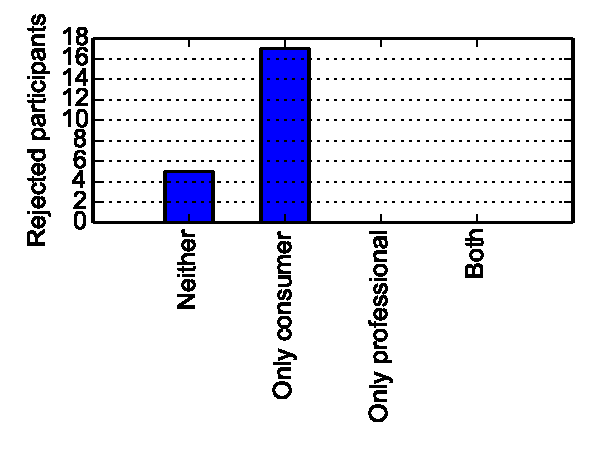
\includegraphics[width=0.5\textwidth]{figs/reject-daw.pdf}
  \caption{Response of rejected participants when asked whether they had
    previously used consumer/professional audio editing software}
  \label{fig:rejectdaw}
\end{figure}

Figure~\ref{fig:rejectvis} plots the number of incorrect responses received for
each visualisation, which shows that no particular visualisation is responsible
for the mistakes. However, Figure~\ref{fig:rejectclip} shows that there is
variation in the mistakes made for each clip, particularly clips 4 and 5. An
analysis of the incorrect in and out points for these clips found that
the mistakes were varied and don't suggest a systematic problem. 

\begin{figure}[ht]
\centering
\begin{subfigure}{.5\textwidth}
  \centering
  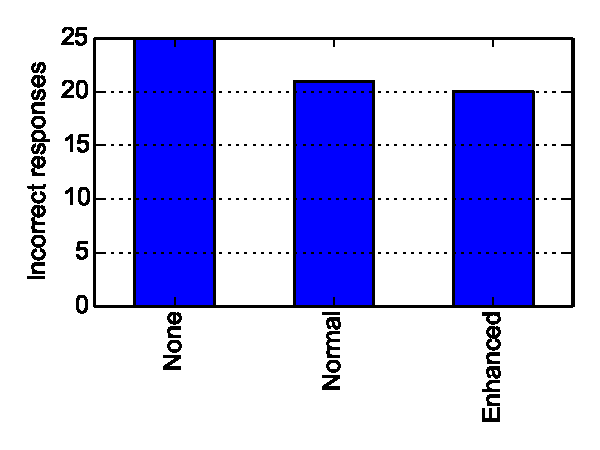
\includegraphics[width=\linewidth]{figs/rejects-vis.pdf}
  \caption{By visualisation}
  \label{fig:rejectvis}
\end{subfigure}%
\begin{subfigure}{.5\textwidth}
  \centering
  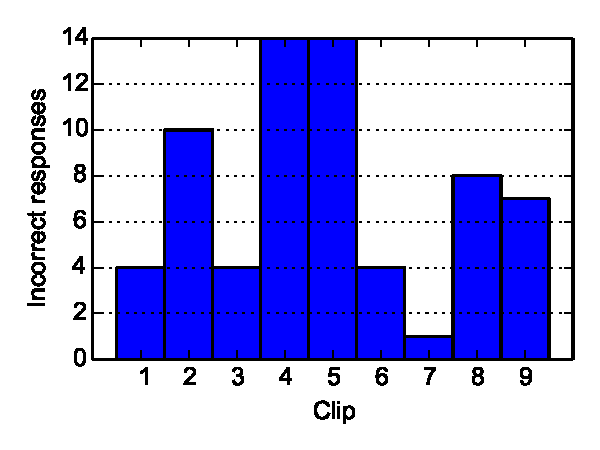
\includegraphics[width=\linewidth]{figs/rejects-clip.pdf}
  \caption{By clip}
  \label{fig:rejectclip}
\end{subfigure}
\caption{Analysis of incorrect responses}
\label{fig:rejects}
\end{figure}

\subsubsection{Demographics}
The demographic of the participants showed a heavy bias (80\%) of male
participants, and a larger proportion in the 26-45 age range (see
Figure~\ref{fig:age}). This reflects the population to which the experiment was
promoted (see Section~\ref{sec:promo}) and is not expected to skew the results.

\begin{figure}[ht]
  \centering
  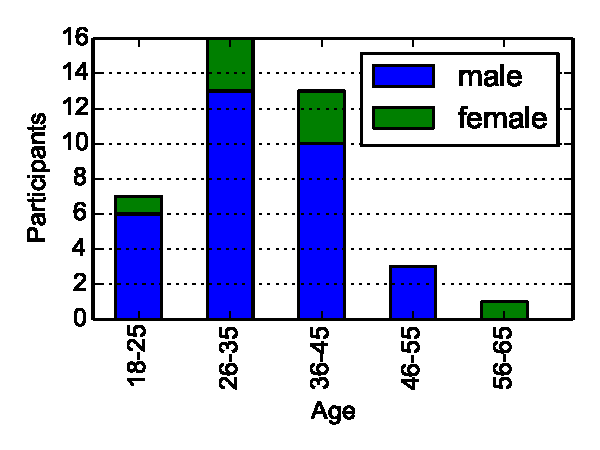
\includegraphics[width=0.5\textwidth]{figs/age.pdf}
  \caption{Age and gender of participants. Male/female ratio was 32/8
    (80\%/20\%). One participant declined to respond to the question.}
  \label{fig:age}
\end{figure}

Most participants had previous experience of using both consumer and
professional audio editing software (see Figure~\ref{fig:experiencedaw}), with
29\% of participants only having experience of consumer software or no
experience at all.

When asked about years of professional audio experience, 39\% of participants
reported having no experience, with the remainder being spread out up to a
maximum of 25 years (see Figure~\ref{fig:experienceyears}). Interestingly, the
answer people gave peaks at the 5 and 10--year marks, where people may have
given a rounded number rather than an accurate figure.

\begin{figure}[ht]
\centering
\begin{subfigure}{.5\textwidth}
  \centering
  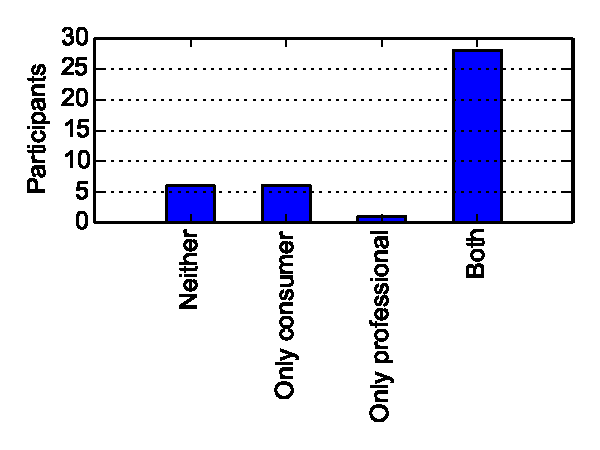
\includegraphics[width=\textwidth]{figs/daw.pdf}
  \caption{Previous use of audio editing software}
  \label{fig:experiencedaw}
\end{subfigure}%
\begin{subfigure}{.5\textwidth}
  \centering
  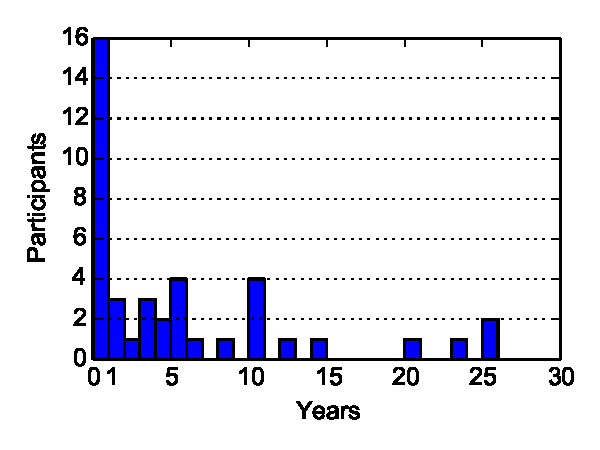
\includegraphics[width=\linewidth]{figs/experience.pdf}
  \caption{Years of professional audio experience}
  \label{fig:experienceyears}
\end{subfigure}
\caption{Response of participants to questions about experience}
\label{fig:experience}
\end{figure}

\subsubsection{Analysis methods}
This section describes the various tools that were used to analyse the data
collected using the experiment, find differences between conditions and
determine whether they are of significance.

\paragraph{Box plot}
A box plot \cite{McGill1978} is a technique used to graph distributions by 
their quartile values (i.e. 25th, 50th and 75th percentiles). An example can be
seen in Figure~\ref{fig:seekbox}. The box extends from the first to the third
quartile, with the second quartile (median) marked as a line through the box.
Lines are drawn from the box to the minimum and maximum, known as `whiskers',
however data determined to be outliers are marked separately as crosses.
The 95\% confidence interval of the median is marked as a notch in the box.

\paragraph{ANOVA}
Analysis of variance is a method of testing whether the mean values of several
groups are equal or not. It assumes that the observations are independent, that
the data have a normal distribution, and that the variance within the groups
are similar. One-way ANOVA tests for a null hypothesis that the means values of
the factors are the same.

\paragraph{Tukey's test}
If the null hypothesis is rejected using ANOVA, we know that there is a
difference between the factors, but we don't know which ones. Tukey's test is a
post-hoc analysis for discovering the difference between individual factors.
It assumes that the observations are independent and that the variance within
the groups are similar.

When Tukey's test is graphed, the mean values are represented by a dot with a
line either side showing the confidence interval. Confidence intervals which
don't overlap can be said to be significantly different.

\paragraph{Standardisation}
Some observations can be biased through participant behaviour. For example,
person A navigates audio recordings by quickly clicking along the timeline
while person B navigates with only a few considered clicks. To block this
factor, the responses of each participant can be standardised so that they have
a mean value of 0 and a standard deviation of 1. This allows the difference
between different participants responses to be measured fairly.

Standardisation maps observations to the `\textbf{standard score}'. This is a
dimensionless unit which represents the number of standard deviations an
observation is above the mean.

\subsubsection{Performance metrics}\label{sec:studymetrics}
An analysis was carried out on the performance metrics that were measured while
participants used the interface (see Section~\ref{sec:measures}).

\paragraph{Seek action}
The number of seek actions made was standardised for each participant. This was
done to reduce variation due to different search styles (i.e. frequent aimless
seeking along the timeline vs. infrequent purposeful seeking)

ANOVA found there to be a difference between the visualizations for $p < 0.01$
and Tukey's HSD test (see Figure~\ref{fig:seektukey}) showed that the number of
seek actions are different for each visualization in favour of the enhanced
version, again for $p < 0.01$. Even without standardisation, the same result
holds for $p < 0.05$.

\begin{figure}[ht]
\centering
\begin{subfigure}{.5\textwidth}
  \centering
  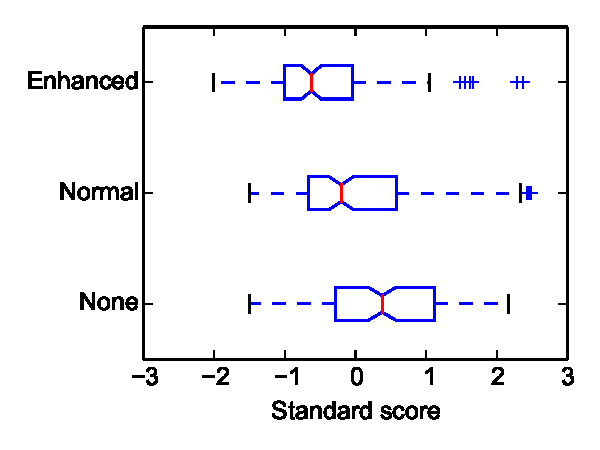
\includegraphics[width=\textwidth]{figs/seek-std.pdf}
  \caption{Box plot}
  \label{fig:seekbox}
\end{subfigure}%
\begin{subfigure}{.5\textwidth}
  \centering
  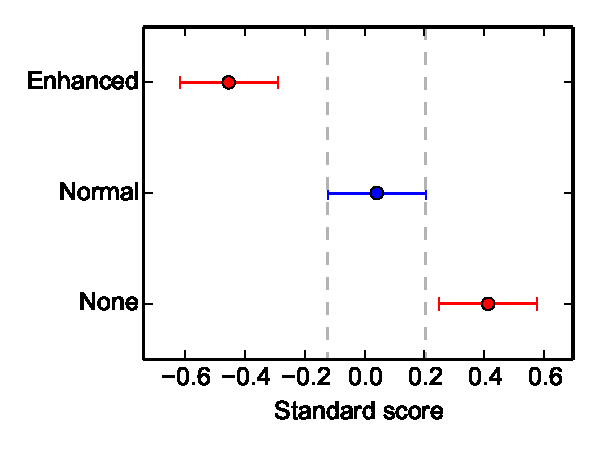
\includegraphics[width=\linewidth]{figs/seek-std-tukey99.pdf}
  \caption{Tukey's test (99\% confidence interval)}
  \label{fig:seektukey}
\end{subfigure}
\caption{Number of seek actions, standardised per participant}
\label{fig:seek}
\end{figure}

\paragraph{Selection time}
The time taken to make a selection was calculated as the difference between the
time the play button was first pressed and the time the final selection was
made. This reduces variation due to participants not starting the task
immediately and participants who made a selection, then checked the rest of the
recording for other pieces of music. The mean and standard deviation of the
selection time was standardised for each participant to reduce the effect of
people's natural pace.

\begin{figure}[ht]
\centering
\begin{subfigure}{.5\textwidth}
  \centering
  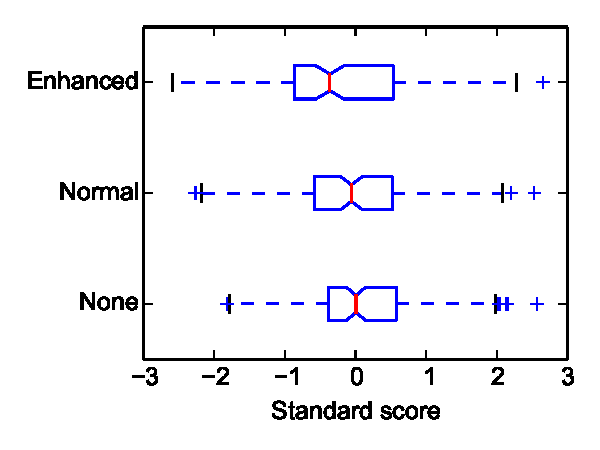
\includegraphics[width=\textwidth]{figs/playstart-to-selectend-std.pdf}
  \caption{Box plot}
  \label{fig:selecttimebox}
\end{subfigure}%
\begin{subfigure}{.5\textwidth}
  \centering
  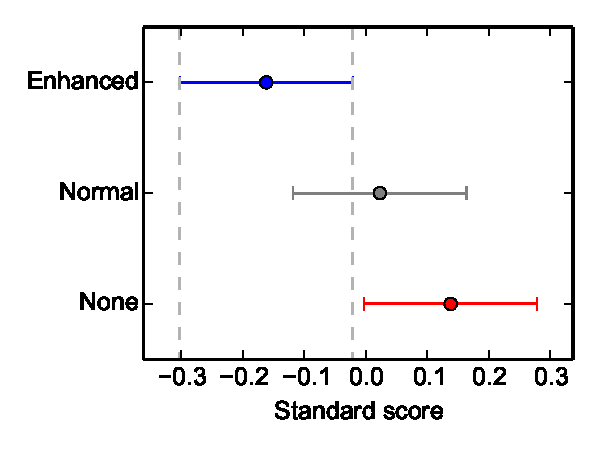
\includegraphics[width=\linewidth]{figs/playstart-to-selectend-std-tukey95.pdf}
  \caption{Tukey's test (95\% confidence interval)}
  \label{fig:selecttimetukey}
\end{subfigure}
\caption{Selection time (time between start of playback and final selection),
    standardised per participant}
\label{fig:selecttime}
\end{figure}

ANOVA showed that there was a significant difference between visualizations for
$p < 0.05$. Tukey's test (see Figure~\ref{fig:selecttimetukey}) found that
there was a difference between no visualization and the enhanced version, but
not between either of them and the normal waveform.

\paragraph{Error}
The absolute error of the selections made by each participant were calculated
for the inpoint, outpoint and sum of both. ANOVA found there to be no
difference between the visualisations for the inpoint or the sum, but found a
significant difference ($p < 0.05$) for the outpoint.  Tukey's test (see
Figure~\ref{fig:outpointerrtukey}) found that the absolute error of the
outpoint for the enhanced visualization was significantly lower than the other
two visualizations, but that the other two were no different.

This is an unexpected result which is difficult to explain, as the inpoint and
sum errors were not even close to rejecting the null hypothesis ($p > 0.3$).
Although the result is significant, the improvement in accuracy is only about
150ms which is small in the context of 5-minute recordings.

\begin{figure}[ht]
\centering
\begin{subfigure}{.5\textwidth}
  \centering
  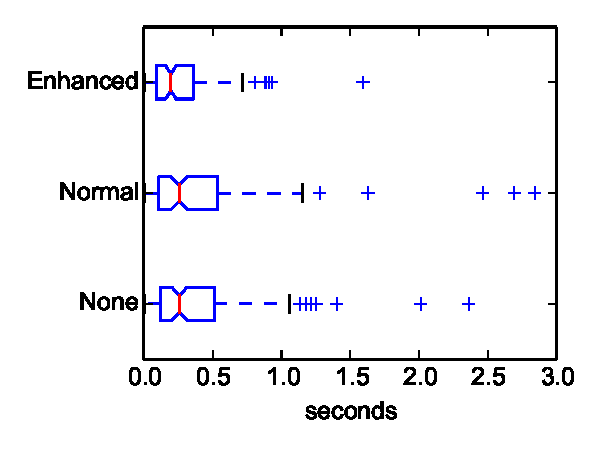
\includegraphics[width=\textwidth]{figs/outpoint-abserr.pdf}
  \caption{Box plot}
  \label{fig:outpointerrbox}
\end{subfigure}%
\begin{subfigure}{.5\textwidth}
  \centering
  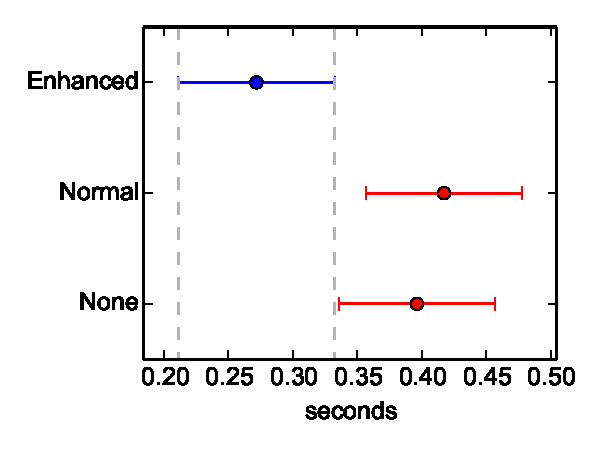
\includegraphics[width=\linewidth]{figs/outpoint-abserr-tukey95.pdf}
  \caption{Tukey's test (95\% confidence interval)}
  \label{fig:outpointerrtukey}
\end{subfigure}
\caption{Absolute error for the outpoint of selections}
\label{fig:outpointerr}
\end{figure}

\paragraph{Zoom}
The experimental interface included two displays -- one overview display
covering the length of the recording, and a zoomed display which showed a
magnified part of that. The number of times the zoom in and zoom out buttons
were pressed was logged. The sum of these values for each visualization is
shown in Figure~\ref{fig:zoomtotal}. By subtracting zoom out from zoom in, we
can infer what the final zoom level was when the response was submitted. The
final zoom levels for each visualization are shown in
Figure~\ref{fig:zoomfinal}.

\begin{figure}[h!]
\centering
\begin{subfigure}{.5\textwidth}
  \centering
  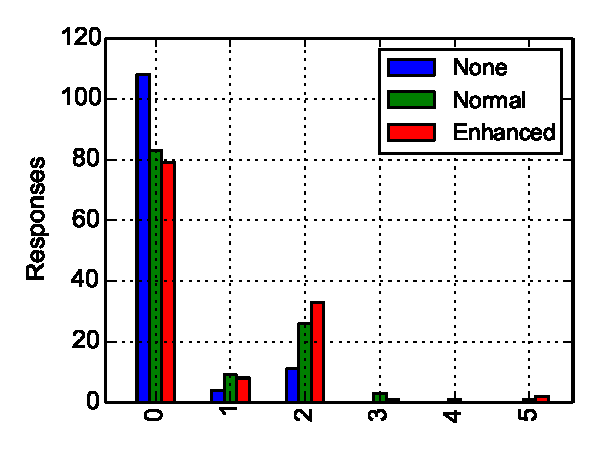
\includegraphics[width=\linewidth]{figs/zoomtotal.pdf}
  \caption{Total zoom actions}
  \label{fig:zoomtotal}
\end{subfigure}%
\begin{subfigure}{.5\textwidth}
  \centering
  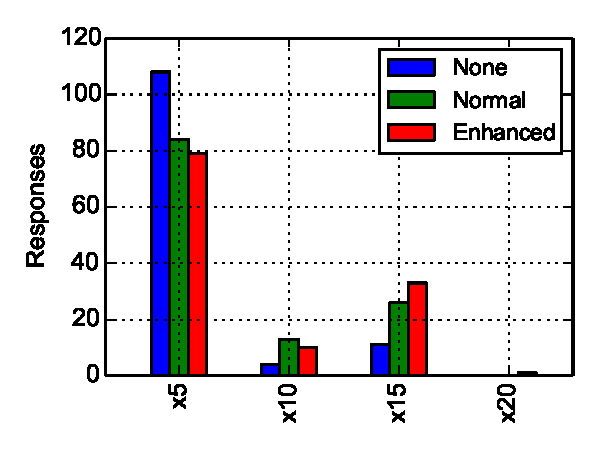
\includegraphics[width=\linewidth]{figs/zoomfinal.pdf}
  \caption{Final zoom level}
  \label{fig:zoomfinal}
\end{subfigure}
\caption{Analysis of zoom usage}
\label{fig:zoom}
\end{figure}

Most of the time, participants didn't touch the zoom controls and opted to leave
it on the default x5 zoom level, which displays roughly one minute of audio
across 1045 pixels ($\sim$50ms per pixel). Other than the x5 level, x15 was
more popular than x10 for all visualizations and x20 was barely used at all.

\subsubsection{Comparison}
Participants were asked to directly compare the three visualizations at the end
of the experiment. The results are shown in Figure~\ref{fig:compare}.

\begin{figure}[ht]
\centering
\begin{subfigure}{.5\textwidth}
  \centering
  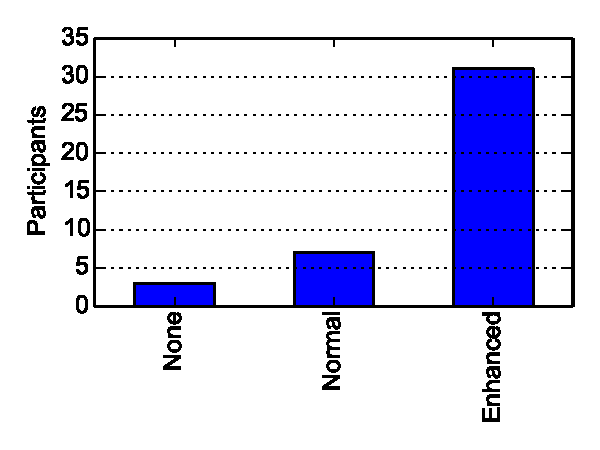
\includegraphics[width=\textwidth]{figs/easiest.pdf}
  \caption{Easiest to use}
  \label{fig:easiest}
\end{subfigure}%
\begin{subfigure}{.5\textwidth}
  \centering
  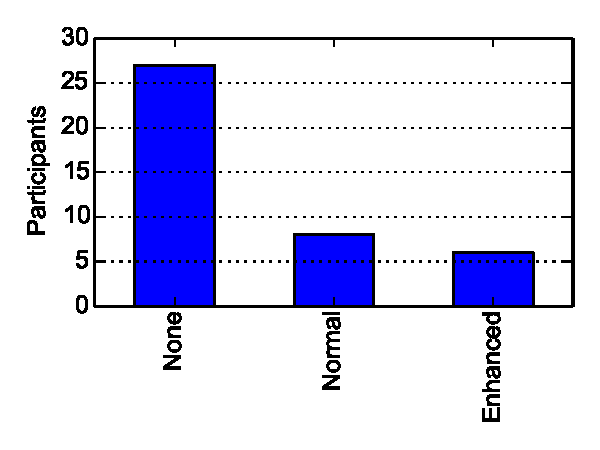
\includegraphics[width=\linewidth]{figs/frustrating.pdf}
  \caption{Most frustrating}
  \label{fig:frustrating}
\end{subfigure}
\caption{Response of participants when asked to compare the visualisations
  using different criteria}
\label{fig:compare}
\end{figure}

A clear majority of 76\% thought that the enhanced waveform was the easiest to
use, with the normal waveform receiving 17\% of votes and 7\% for no waveform.
The strong preference for the enhanced waveform over the others shows that
participants thought the additional information added using colour made their
task easier.

Having no waveform was considered by two-thirds of participants to be the most
frustrating condition, followed by the normal waveform at 20\% and enhanced
waveform at 15\%. Although this is another strong result in favour of using
waveforms, the results are not quite as strong as the ones on ease of
use. It is possible that the false positives and negatives present in the
enhanced waveform caused some people to select it as the most frustrating.

\subsubsection{Task load index}
The TLX responses were standardised to account for variation in the way
different people assign scores. The distributions of the standardised scores
for each visualization are shown in Figure~\ref{fig:tlx}.

\begin{figure}[p]
  \centering
  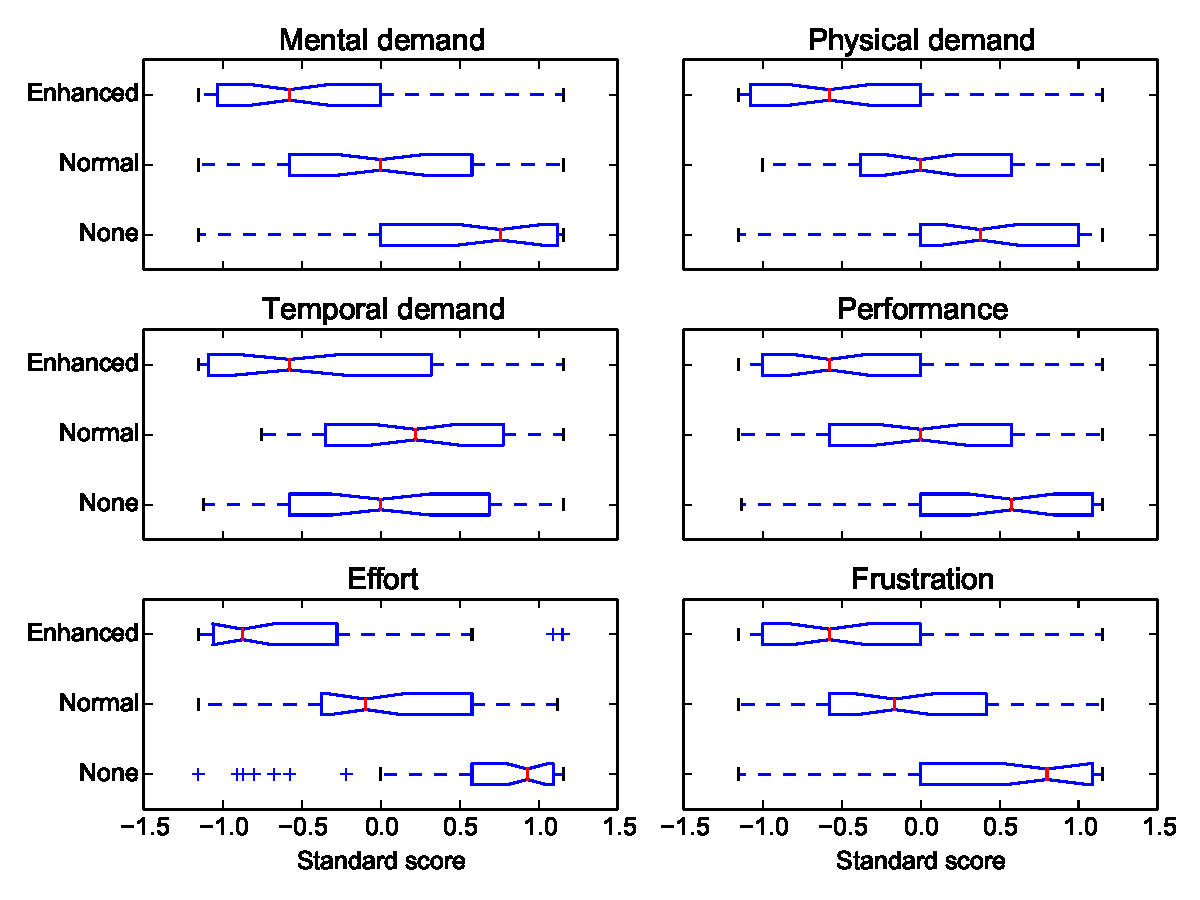
\includegraphics[width=\textwidth]{figs/tlx-std.pdf}
  \caption{Standard score of NASA Task Load Index responses for each
    visualization, standardised per participant.}
  \label{fig:tlx}
\end{figure}

\begin{figure}[p]
  \centering
  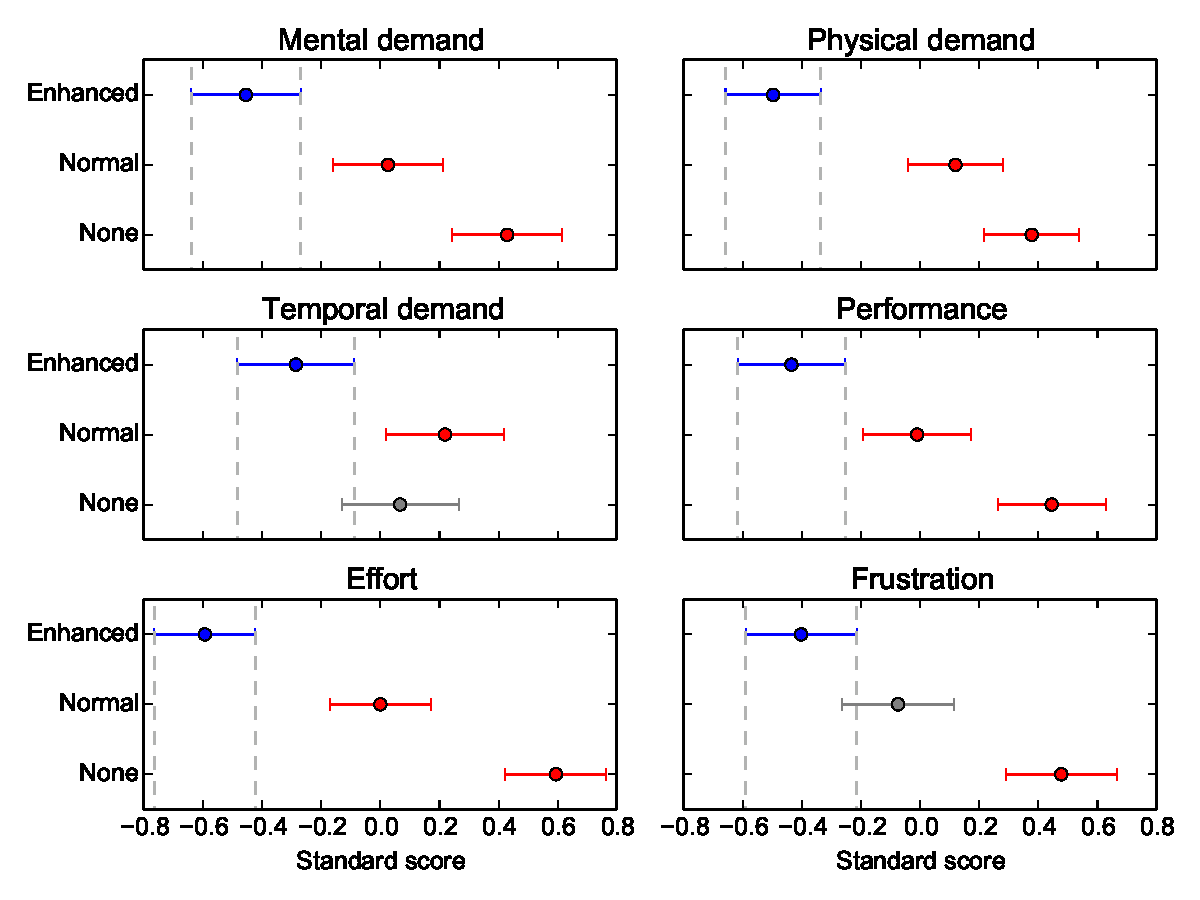
\includegraphics[width=\textwidth]{figs/tlx-std-tukey95.pdf}
  \caption{Standard score of NASA Task Load Index responses for each
    visualization, standardised per participant.}
  \label{fig:tlxtukey}
\end{figure}

ANOVA found there to be significant differences between the visualizations in
all TLX metrics for $p < 0.01$. Tukey's test (see Figure~\ref{fig:tlxtukey})
found that for $p < 0.05$, the enhanced waveform outperformed no waveform in
all metrics except temporal demand, and outperformed the normal waveform in
all metrics except frustration. The normal waveform outperformed no waveform in
mental demand, performance, effort and frustration.

Some scepticism should be given to the physical and temporal demand metrics, as
it's not entirely clear what is meant by that terminology in the context of the
task. Participants are not working against the clock, not are they doing
anything other than moving the mouse. Although some participants may consider
fewer clicks of the mouse to represent reduced physical demand, we cannot
assume that others thought the same.

\subsubsection{Interaction behaviour}
This section looks at how participants used the features available in the
online audio interface, full described in Section~\ref{sec:iface}.
%Informal observation of some participants as they completed the experiment
%revealed that some people used the interface in different ways. For example,
%when one participant had completed their selection, they scanned through the
%remaining unselected content to check that there were no other pieces of music.

\begin{figure}[p]
\centering
\begin{subfigure}{.5\textwidth}
  \centering
  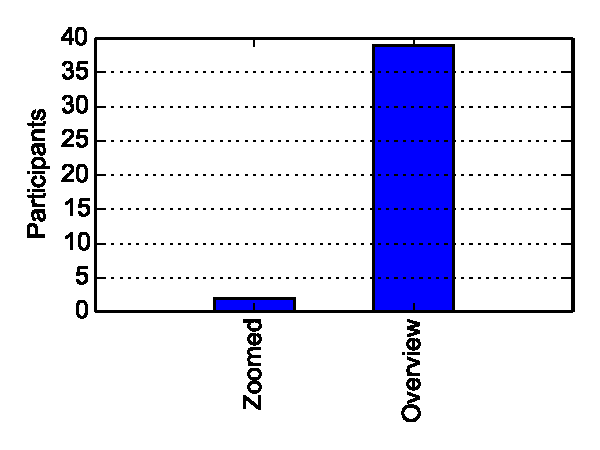
\includegraphics[width=\linewidth]{figs/top-v-bot-pref.pdf}
  \caption{Display}
  \label{fig:displaypref}
\end{subfigure}%
\begin{subfigure}{.5\textwidth}
  \centering
  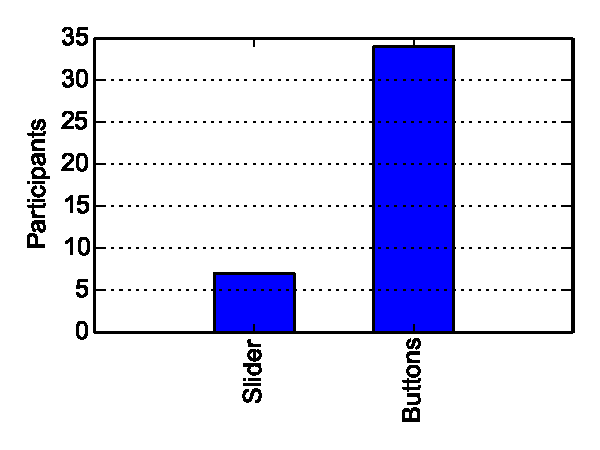
\includegraphics[width=\linewidth]{figs/mark-v-slide-pref.pdf}
  \caption{Selection method}
  \label{fig:selectpref}
\end{subfigure}
\caption{Preference of participants}
\label{fig:pref}
\end{figure}

\paragraph{Top/bottom display}
There are two displays that make up the interface -- a zoomed display at the
top and an overview display on the bottom. Either of the displays can be used
to navigate the recording and make selections.

For each participant, the number of tasks where they used the zoom display more
than the overview (and vice-versa) were counted. Figure~\ref{fig:displaypref}
shows number of participants who, on average, used the zoomed or overview
display more.

The results show a clear preference for using the overview display more than
the zoom display. Coupled with the results of zoom usage in
Section~\ref{sec:studymetrics}, we can see that for this task most people opted
just to work in the overview display, despite only having a resolution of
roughly 300ms per pixel.

An analysis of the overview and zoom display's usage between different
visualization methods did not find any notable difference.

\paragraph{Selection method}
The design of the interface gave participants two methods of making a selection
-- buttons to mark in and out points using the cursor, and a slider where the
in and out points could be dragged around. The cursor can be moved around in
both the overview and zoomed displays, whereas the slider is only available at
the x1 zoom level. This makes the buttons more useful for fine edits, where
high precision is needed. When using the slider, the selection display updates
as you move it making it easier for people to see where their selection is.

For each response, the method with the most actions was found and these
preferences were summed for each participant to calculate their overall
preference. The results are shown in Figure~\ref{fig:selectpref}.

The buttons were the most popular method of making a selection, with only 17\%
of people using the slider more. Informal feedback found that some people has a
strong preference for using the slider but were frustrated that there wasn't a
second slider available on the zoomed display.

